\section{Tutorial}
\label{tutorial_b}

The objective of this chapter is to get you to a stage where you can use BMotion Studio to visualize Event-B or Classical-B models. 
We expect that you have already downloaded the BMotion Studio tool (see Section~\ref{installation}).
 
%We expect you to have a basic understanding of logic and an idea why doing formal modelling is a good idea.  
You should be able to work through the tutorial with no or little outside help.
We encourage you not to download solutions to the examples but instead to actively build them up yourself as the tutorial progresses.
If something is unclear, remember to check the Reference (\ref{reference_b}) for more information.

\subsection{Preparation}

Let's start by creating a new visualization template as described in Section~\ref{vis_template}.
Just download the \file{bms-b-template.zip}{predefined template}, decompress the archive and rename the folder to \texttt{lift}.
%After refreshing your browser, a new folder called \texttt{lift} should appear in your workspace (see Figure~\ref{fig_tut_01_workspace}).

%\subsection{Creating a new visualization Template}
%
%Let's start by creating a new visualization template.
%The easiest way to create a new visualization template is to duplicate the default template \texttt{b\_template} that is included in the \texttt{workspace} folder of your \bms~installation.
%Just duplicate the \texttt{b\_template} folder and rename it to \texttt{lift}.
%After refreshing your browser, a new folder called \texttt{lift} should appear in your workspace (see Figure~\ref{fig_tut_01_workspace}).
%Navigate to the \texttt{lift} folder. 
%The folder contains three files:
%\begin{itemize}
%\item \texttt{template.html}: The HTML file is the root file of your visualization. It contains the actual visualization and it's configuration.
%\item \texttt{template.groovy}: The Groovy script file is the place where the user can communicate with the formal model by means of the ProB Java API\footnote{\url{http://www.stups.hhu.de/ProB/index.php5/ProB_Java_API}}.
%For instance, the user may register methods that can be called in the JavaScript file.
%%The Groovy script file is the place where you can setup the communication between your visualization and the ProB animator.
%%In particular, the Groovy script file is the link between the formal model and the visualization.
%%It allows you to programmatically control the ProB animator and to access the actual formal model being visualised.
%%In addition, you can register functions that can be called from the visualization, e.g. executing an Event-B event after pressing a button in the visualization.
%\item \texttt{template.js}: In the JavaScript file you can setup observers and actions.
%Moreover, the user can take advantage of the entire JavaScript language.
%There exist are a lot of libraries for JavaScript that you can apply to create custom visualizations.
%For instance, it exists libraries for manipulating the DOM of an HTML document, or for generating chart and plot diagrams.
%%In addition, you can call functions that are registered in the Groovy script file.
%%This enables you to add some interactivity to your visualization.
%%For instance, pressing a button in your visualization could cause the execution of an Event-B event.
%\end{itemize}
%
%\begin{figure}[!ht]
%\begin{center}
%	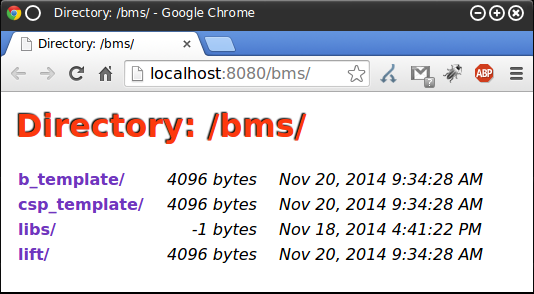
\includegraphics[width=12cm]{img/tutorial/tut_01.png}
%	\caption{\bms~Workspace}
%	\label{fig_tut_01_workspace}
%\end{center}
%\end{figure}

\subsection{The Formal Model}

We are going to create a visualization	for a simple lift system that allows movement of a single lift cage between three floors.
The door of the lift can be closed and opened - all in response to the pressing of floor call and cage send buttons.

You can download the Event-B model \file{EventBLift.zip}{here}.
Decompress the archive and put the files into a new folder called \texttt{model} relative to your \texttt{template.html} file.

\subsection{Link the Model with the Visualization}

The first step consists of linking the model with the visualization.
For this, open the \texttt{bmotion.json} file with an editor of your choice and set the \textit{model} path property to ``model/MLift.bcm''.
This links the visualization with the Event-B machine called ``MLift''.
Linking a model within the \texttt{bmotion.json} file will automatically load the model, when starting the visualization (see Section~\ref{sec:stat_vis}).

\subsection{Create the Actual Visualization}

Please download the prepared \file{lift.svg}{lift.svg} file and open it with Inkscape as demonstrated in Figure~\ref{fig_tut_02_inkscape}.
Feel free to modify and explore the SVG graphic.
In order to link graphical elements of the SVG graphic with the formal model later, we have to give them identifiers. 
For this, select an element in Inkscape, open the context menu and select \textsf{Object Properties}.
A popup window should be opened as demonstrated in Figure~\ref{fig_tut_02_inkscape}.
As an example, we give the graphical element that represents the door (the gray filled rectangle), the id ``door''.
In Section~\ref{sec_creation_observers} we explain how we can use this information in order to establish \textit{observers}.
If you are satisfied with your SVG graphic, save it as a plain SVG graphic with \textsf{File $\rangle$ Save As}.
Select \textsf{Plain SVG (*.svg)} as an output format and click on the \textsf{Save} button.
You can save the SVG file anywhere on your local system. 
Open the SVG file with an editor of your choice, copy the SVG code and paste it within the body tag in the \texttt{template.html} file.

\subsection{Start the Visualization}
\label{sec:stat_vis}

Let's try out the visualization for the first time!
Just drag and drop the \texttt{bmotion.json} file on the marked area or open it via the file dialog.
%In your browser, navigate to the folder \texttt{lift} folder and click on the \texttt{template.html} file.
The visualization should start.
At the right bottom you will find a menu called \textsf{ProB} for opening different ProB related views.
For instance, Figure~\ref{fig_tut_03_running1} shows the running lift visualization with the ProB Events view opened.

At the moment nothing spectacular happens when changing the state (i.e. executing events in the Event view) as no observers exist yet.
In the next Section we learn how we can link graphical elements with the formal model by establishing observers.

\begin{figure}[!ht]
\begin{center}
	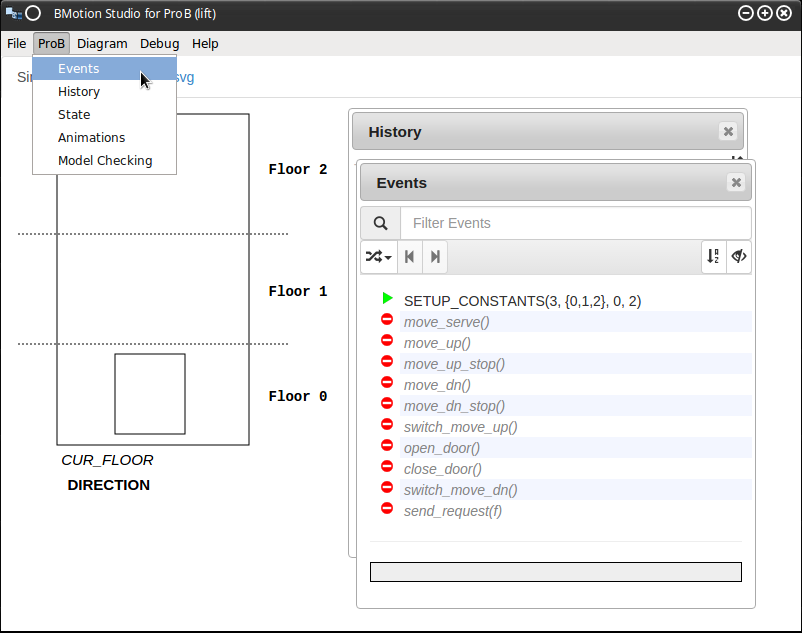
\includegraphics[width=12cm]{img/tutorial/tut_03.png}
	\caption{Running the Lift visualization for the First Time}
	\label{fig_tut_03_running1}
\end{center}
\end{figure}

\subsection{Create Observers}
\label{sec_creation_observers}

Observers are used to link graphical elements with the model. 
An observer is notified whenever the model has changed its state, i.e. whenever an event has been executed. 
In response, the observer will query the model's state and triggers actions on the linked graphical elements in respect to the new state.
In general, observers are defined in the JavaScript file and should be places in the \texttt{script.js} file. 
As an example, consider the following \textit{formula observer}:

\begin{lstlisting}[language=JavaScript, caption={Formula Observer Displaying the Current Floor (JavaScript)}]
bms.observe("formula", {
  selector: "#txt_cur_floor",
  formulas: ["cur_floor"],
  trigger: function (origin, result) {
    origin.text(result[0])
  }
});
\end{lstlisting}

\info{Checkout Section~\ref{b_observers} for more details about observers.}

We are going to explain the JavaScript code line by line.
In line 1 we register a formula observer on the graphical element with the id \textit{txt\_cur\_floor} (line 2) that is located in our \texttt{template.html} file.
%Line 1 means that we want to transform the graphical element with the id \textit{txt\_cur\_floor} that is located in our \texttt{index.html} file.
\bms~follows the jQuery selector syntax\footnote{For more information about jQuery and selectors we refer the reader to the jQuery
API documentation http://api.jquery.com/category/selectors/.} to select graphical elements.
The prefix ``\#'' denotes that we want to select an element by its id.
In line 3 we define a list of observed formulas.
In this case we observe the variable \textit{cur\_floor}.
In line 4 to 6 we define a trigger function that is called after every state change with its \textit{origin} (the origin parameter holds a reference to the graphical element that the observer is attached to) and the \textit{result} (the result parameter contains the results of the defined formulas in an array, e.g. use \textit{result[0]} to obtain the result of the first formula).
The trigger function changes the text of the graphical element (\textit{origin}) to the current value of the variable \textit{cur\_floor} (\textit{result[0]}).
%Reload the visualization by clicking on the \texttt{Reload} button and play with the visualization by executing some events.
%Line 2 affects that the attribute \textit{text} will be set to the value that is returned by the followed closure.
%In particular, the closure evaluates the expression \textit{cur\_floor} in the current state and returns the value to be set.
%In other words, the observer sets the current value of the variable \textit{cur\_floor} into the visual text element with the id \textit{txt\_cur\_floor}.
%Line 3 is responsible to register the observer.
%All registered observer will be triggered after every state change.

Let's create another observer.
Check out the following JavaScript snippet:

\begin{lstlisting}[language=JavaScript, caption={Formula Observer for the Lift Door (JavaScript)}]
bms.observe("formula", {
  selector: "#door",
  formulas: ["cur_floor", "door_open"],
  trigger: function (origin, result) {
    
    switch (result[0]) {
      case "0":
        origin.attr("y", "175");
        break;
      case "1":
        origin.attr("y", "60");
        break;
      case "-1":
        origin.attr("y", "275");
        break;
    }
    
    if(result[1] === "TRUE") {
      origin.attr("fill", "white");
    } else {
      origin.attr("fill", "lightgray");
    }
    
  }
});
\end{lstlisting}

In line 1 we register a formula observer on the graphical element that matches the selector ``\#door'' (line 2) (similar to the previous defined formula observer).
%Line 1 means that we want to transform the graphical element with the id \textit{door}, similar to the previous observer.
In line 3 we define the set of observed formulas (\textit{cur\_floor} and \textit{door\_open}).
In line 4 to 24 we define a trigger function, that makes the following action:
Line 5 to 15 will switch the \textit{y} coordinate of the door (denoting the movement of the door between floors) according to the current value of the variable \textit{cur\_floor} (\textit{result[0]}).
Lines 18 to 22 affect that the attribute \textit{fill} of the door will be set to ``white'' (denoting the door is open) whenever the formula \textit{door\_open} evaluates to \textit{TRUE} in the current state (\textit{result[1]}), otherwise to ``lightgray'' (denoting the door is closed).
%Whenever the expression \textit{door\_open} evaluates to \textit{TRUE}, the value \textit{white} (denoting the door is opened) is returned, otherwise the value \textit{lightgray} (denoting the door is closed) is returned.
%Line 3 to 17 will switch the \textit{y} coordinate of the door (denoting the movement of the door between floors) according to the evaluation result of the expression \textit{cur\_floor}.
%In line 18 we register the observer.
%You can use the entire Groovy power and feature range for defining your observers.

Add both snippets to your \texttt{script.js} file, save the file and click on the \texttt{Reload} button.
Let's see how this affects our visualization:
Setup and initialize the machine using the ProB events view.
Execute some events and see what happens.
For instance, Figure~\ref{fig_tut_04_running2} shows the lift visualization where the lift is on floor 0 and the door is open.

\begin{figure}[!ht]
\begin{center}
	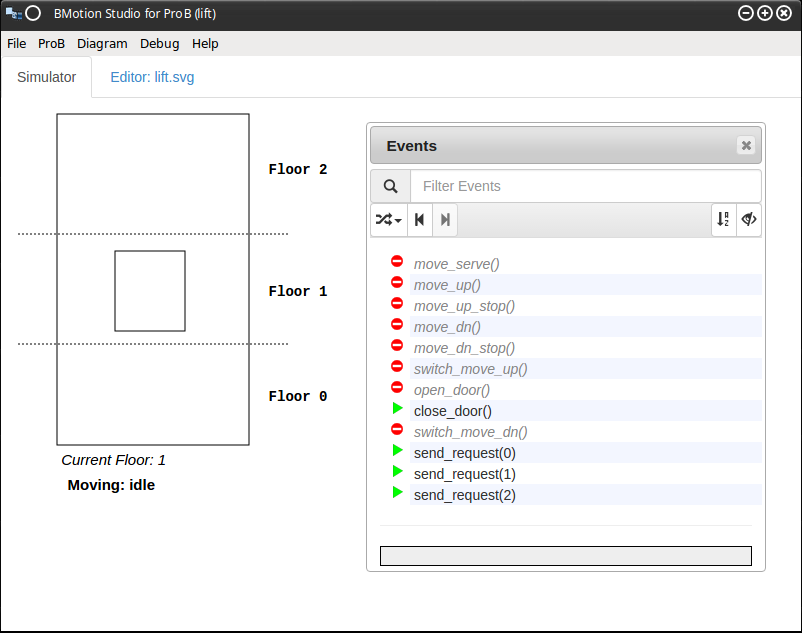
\includegraphics[width=12cm]{img/tutorial/tut_04.png}
	\caption{Lift visualization with observers}
	\label{fig_tut_04_running2}
\end{center}
\end{figure}

\subsection{Add Event Handler}

In this Section we learn how we can enhance our visualization with interactive features, e.g. executing an Event-B event by clicking on a graphical element.

Let's add an interactive feature, where the user can click on a floor label to order the lift on the corresponding floor.
Add this code snippet to your \texttt{script.js} file:
\newpage
\begin{lstlisting}[language=JavaScript, caption={Example of an Interactive Feature (JavaScript)}]
bms.executeEvent({
  selector: "text[data-floor]",
  events: [
    {
      name: "push_call_button", 
      predicate: function (origin) {
        return "b=" + $(origin).attr("data-floor")
      }
    }
  ]
});
\end{lstlisting}

%For instance, clicking on the floor Label ``Floor 1'' should execute the Event-B event \textit{push\_call\_button(1)}.
In line 1 we register an execute event handler for each graphical element that matches the defined selector ``text[data-floor]'' (line 2).
In particular, the selector matches the three floor labels (see Figure~\ref{fig_tut_03_running1}).
In line 3 to 10 we define the list of events that should be wired with the graphical elements.
Every event should contain the \textit{name}.
In addition, the user may enter a \textit{predicate} that defines the event's arguments.
If the user defines more than one event, a tooltip will be shown with a list of the defined events after clicking on the graphical element.
In our example we define only one event with the \textit{name} $push\_call\_button$ and the \textit{predicate} that is determined by a closure that passes a reference to the element (\textit{origin}).
In particular, we use the value of the attribute \textit{data-floor} of the corresponding floor label (\textit{origin}) to define the event parameter (line 6).

Apply these changes by clicking on the \texttt{Reload} button and try to click on a floor label.
This should call the Event-B event \textit{push\_call\_button} with the corresponding predicate/parameter.

Let's add another interactive feature, where the user can click on the graphical element that represents the door to open or close the door respectively.
%The first step consists of registering a new Groovy function that executes the corresponding event \textit{open\_door} or \textit{close\_door}.
%Add the code snippet to your \texttt{template.groovy} file:
%\begin{lstlisting}[language=Groovy, caption={Registering a Groovy Function (Groovy)}]
%bms.registerMethod("openCloseDoor", {
%    def Trace t = bms.getTool().getTrace()
%    def Trace newTrace = executeEvent(t, "open_door", []) ?: executeEvent(t, "close_door", [])
%    if (newTrace != null) {
%        animations.traceChange(newTrace)
%        return [newState: newTrace.getCurrentState().id]
%    }
%})
%
%def Trace executeEvent(t,name,pred) {
%    try {
%        t.execute(name, pred)
%    } catch(IllegalArgumentException e) {
%        null
%    }
%}
%\end{lstlisting}
%In Line 1 we register a new Groovy function called \textit{openCloseDoor}.
%The next lines show an example how we can use the ProB Java API.
%In Line 2 we get the current trace of the animation.
%In Line 3, we first try to execute the \textit{open\_door} event by means of a helper method called \textit{executeEvent} (Line 10 to 16).
%If the return value of the helper method is null (the event could not be executed), we try to execute the event \textit{close\_door}.
%If we success (we executed one of the both events), we trigger a trace change, causing to refresh the current animation (Line 5).
%This in turn changes the state and triggers our registered observers.
%Line 6 returns a Json object that contains the state id of the new state.
%This information can used later at the JavaScript side after executing the registered \textit{openCloseDoor} method.
%Let's switch to the JavaScript side.
Add the following code snippet to your \texttt{script.js} file:
%\begin{lstlisting}[language=JavaScript, caption={Call openCloseDoor Groovy Method (JavaScript)}]
%$("#door").click(function () {
%	bms.callMethod("openCloseDoor", {
%		callback: function (data) {
%			console.log("Callback: " + data)
%		}
%	})
%}).css("cursor", "pointer")
%\end{lstlisting}
\begin{lstlisting}[language=JavaScript, caption={Interaction with the Lift Door (JavaScript)}]
bms.executeEvent({
  selector: "#door",
  events: [
    { name: "close_door" }, 
    { name: "open_door" }
  ]
});
\end{lstlisting}

%In line 1 we register a new execute event handler on the graphical element with the id ``door'' (line 2).
%In line 3 to 6 we define two events.
The execute event handler first tries to execute the event \textit{close\_door}.
In case the event is disabled, it tries to execute the next event \textit{open\_door}.
%Line 2 calls our registered Groovy method \textit{openCloseDoor}.
%In Line 3 to 5 we pass a callback function that is called after an event (\textit{open\_door} or \textit{close\_door}) was executed.
%In this case we print the returned new state id on the console.

%These are only small examples for adding interactivity to your visualization.
%You are not limited to these examples.

\subsection{Final visualization}

You can download the final visualization \file{LiftVisualisation.zip}{here}.
